% ---------------------------------------------------------------------------- %

\section{Arquitetura do Sistema}

Por fim, procedeu-se à modelação da arquitetura interna do sistema. Neste capítulo estabelece-se a divisão do sistema em camadas, sendo que os próximos dois capítulos detalham esta modelação.

\label{cap:arquitetura}
O sistema será dividido em três camadas principais:
\begin{enumerate}
    \item a \emph{View} que irá englobar tudo o que será necessário para a apresentação do sistema ao utilizador;
    \item o \emph{Model} que representa a camada de negócios do sistema, esta camada irá fornecer a informação necessária para a canada de apresentação;
    \item a \emph{Data} que representa os objetos de acesso à base de dados, estando cada um deles dependentes da existência do objeto respondente na camada de negócios.
\end{enumerate}

\begin{figure}[ht]
  \centering 
  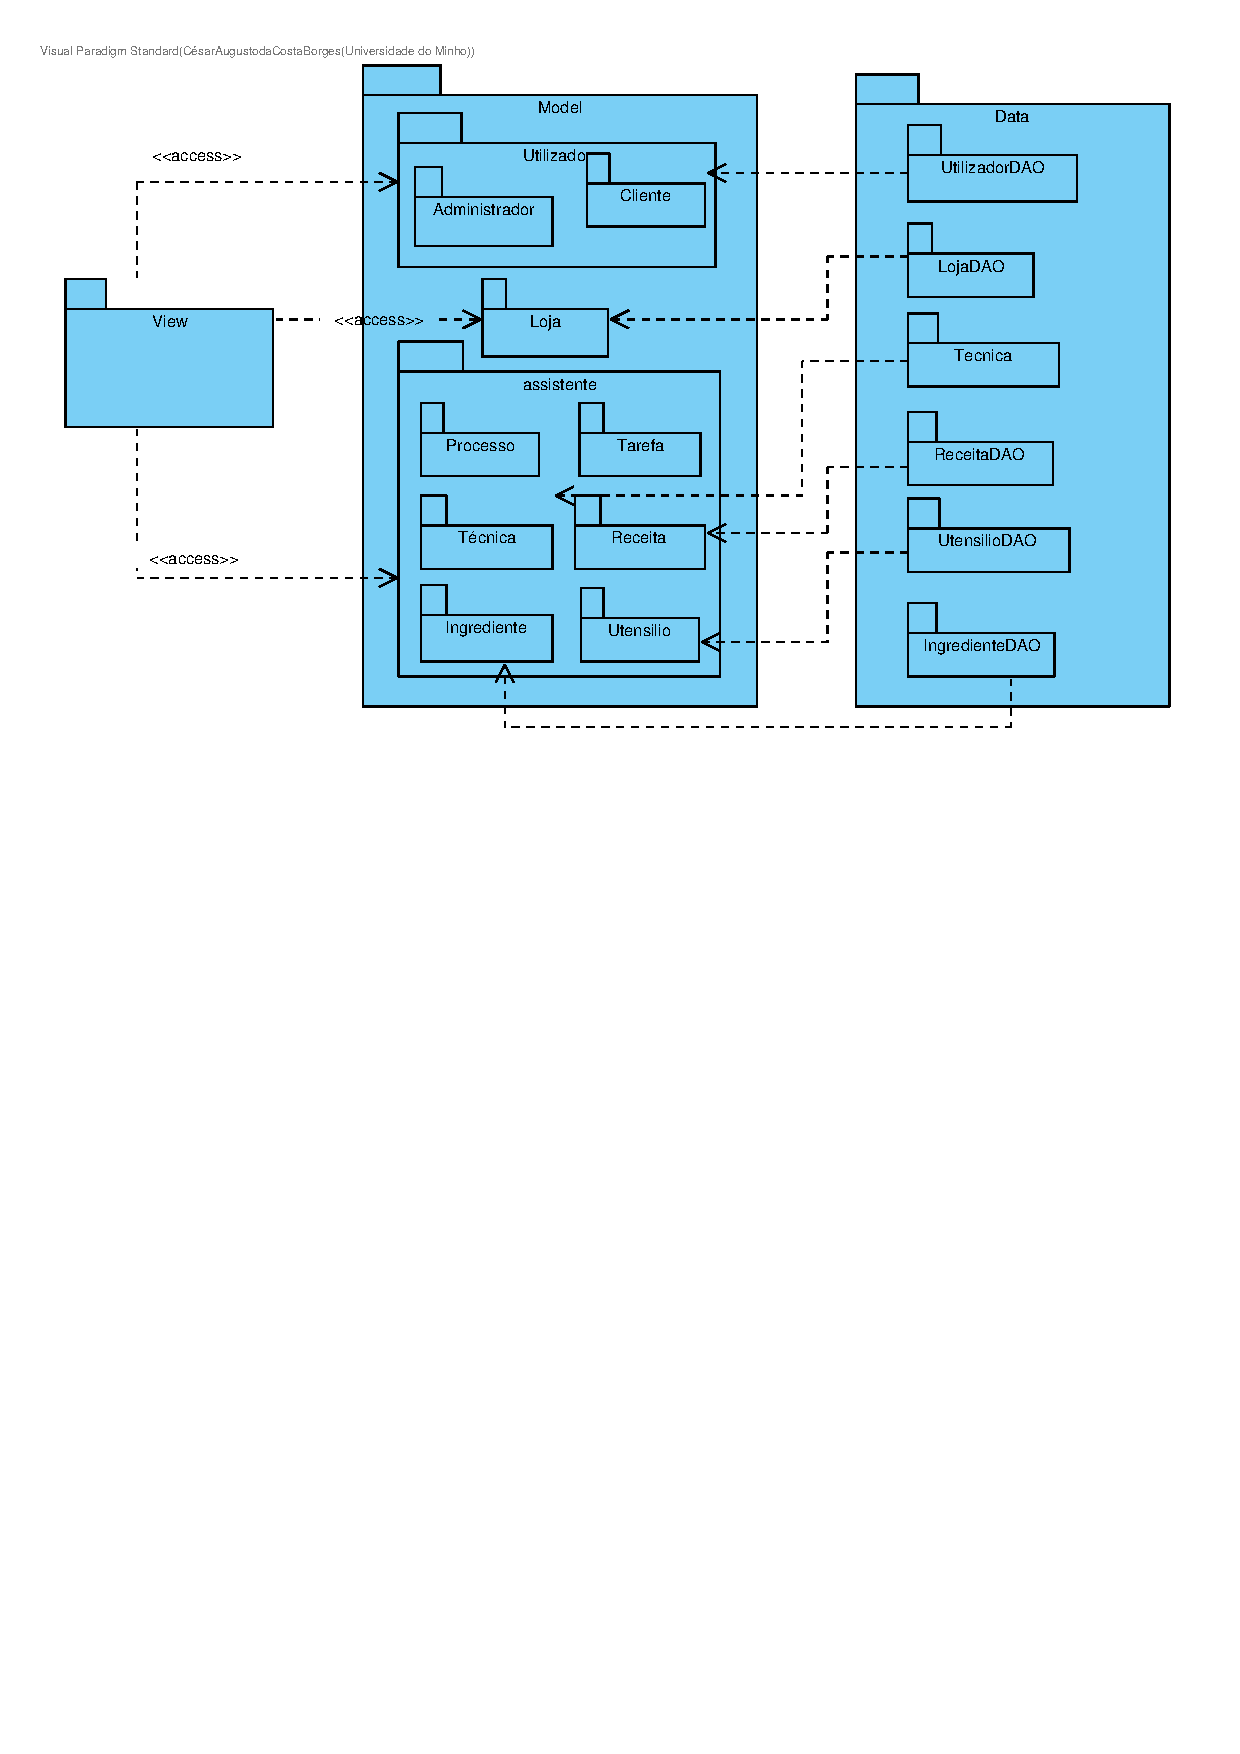
\includegraphics[width = \textwidth]{figures/08/diagrama-Pacotes.pdf}
  \caption{Diagrama de pacotes do sistema.}
  \label{fig:arquitetura:DiagramaPacotes}
\end{figure}

A camada de negócios ainda é dividida em três sub-pacotes:
\begin{enumerate}
    \item \emph{Utilizador} que está relacionado com  representação de todos os dados do utilizador;
    \item \emph{Loja} que representa os dados das lojas;
    \item \emph{Assistente} que está relacionado com o que os dados que o assistente manipulará na confeção das receitas
\end{enumerate}

%  - Arquitetura em 3 camadas
%  Relativamente à arquitetura do sistema irá ser utilizada um arquitetura em três camadas 
  
%  - Diagramas de Instalação
  
%  - Diagramas de Componentes
  
%  - (Diagramas de Pacotes)

%\begin{figure}[ht]
%  \centering
%  \includegraphics[width=\textwidth]{figures/08/pacotes.pdf}
%  \caption{Diagrama de pacotes.}
%  \label{fig:arquitetura:DiagramaPacotes}
%\end{figure}

% ---------------------------------------------------------------------------- %
